\input{preambuloSimple.tex}
\title{	
	\normalfont \normalsize 
	\textsc{{\bf Ingeniería de Servidores (2016-2017)} \\ Grado en Ingeniería Informática \\ Universidad de Granada} \\ [25pt] % Your university, school and/or department name(s)
	\horrule{0.5pt} \\[0.4cm] % Thin top horizontal rule
	\huge Instalación de sistemas operativos y configuración en RAID \\ % The assignment title
	\horrule{2pt} \\[0.5cm] % Thick bottom horizontal rule
}

\author{Manuel Jiménez Molina} % Nombre y apellidos

\date{\normalsize\today} % Incluye la fecha actual

%----------------------------------------------------------------------------------------
% DOCUMENTO
%----------------------------------------------------------------------------------------

\begin{document}
	
	\maketitle % Muestra el Título
	
	\newpage %inserta un salto de página
	
	\tableofcontents % para generar el índice de contenidos
	
	\listoffigures
	
	\listoftables
	
	\newpage
	
	%NOTA: en caso de problema al compilar, compruebe que tiene el paquete: texlive-babel-spanish.noarch  \\
	
	
	
	
	\newpage
	
	%----------------------------------------------------------------------------------------
	%	Cuestión 1
	%----------------------------------------------------------------------------------------
	
	\section{¿Qué modos y/o tipos de “virtualización” existen? (no más de tres párrafos)}
	
	\begin{itemize}
		\item Hipervisor. Hay 2 tipos:
		\begin{itemize}
			\item Tipo 1(nativo):
			Ejecutado en\cite{primero} modo kernel gestiona las llamadas al sistema del sistema operativo invitado (después de que tras esa llamada se produzca una interrupción) de la máquina virtual que se ejecuta realmente en modo usuario, de manera que emula al hardware real.
			
			
			
			\item Tipo 2 (hosted): VMware fue el primero de estos, se ejecuta como usuario sobre un SO anfitrión y ya permite instalar SO invitados sobre VMware. Las llamadas sensibles de los SO invitados se sustituyen por llamadas a procedimiento y el hipervisor las emula.
		\end{itemize}
		
		\item Paravirtualizacion. Los sistemas operativos invitados cuando realizan llamadas al sistema lo que realmente hacen son llamadas al hipervisor que contiene una API con los que manejarlos.
	\end{itemize}
	
	
	%----------------------------------------------------------------------------------------
	%	Cuestión 2
	%----------------------------------------------------------------------------------------
	
	\section{Muestre los precios y características de varios proveedores de VPS (Virtual Private Server)  y compare con el precio de servidores dedicados (administrados y no administrados). Comente diferencias.}
	
	
	La empresa Cyberneticos proporciona los siguiente servidores VPS\cite{cincuentaycuatro} y servidores dedicados\cite{cincuentaycinco}:
	
	\begin{figure}[H] 
		\centering
		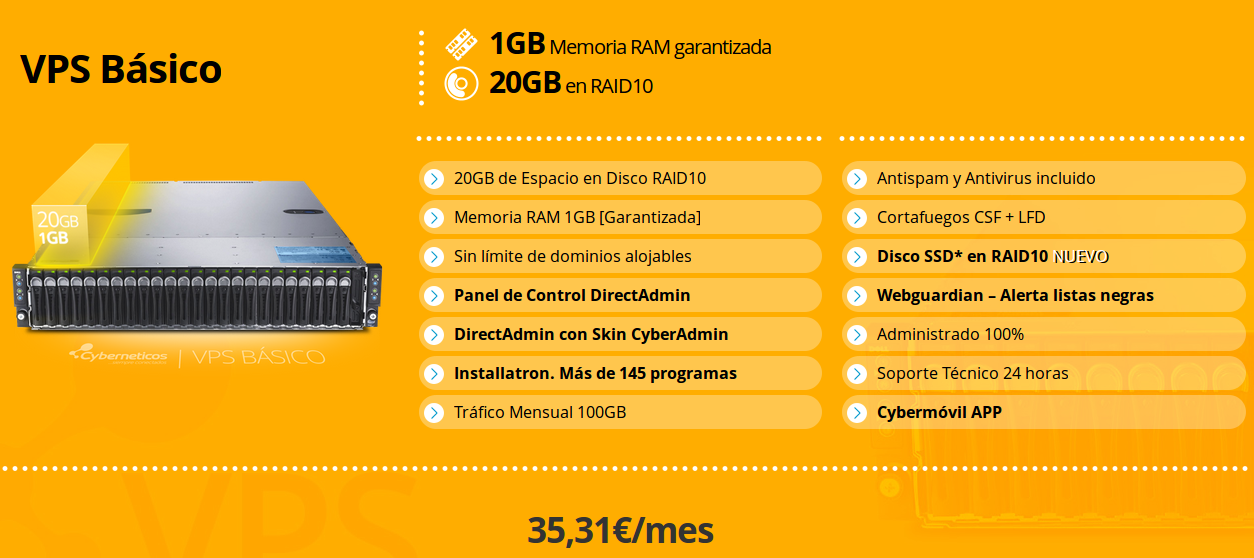
\includegraphics[scale=0.3]{ejercicio2-cyberneticos-1.png} 
		\label{figura1} 
		
		\caption{Cyberneticos,VPS básico} 
	\end{figure}
	
	\begin{figure}[H] 
		\centering
		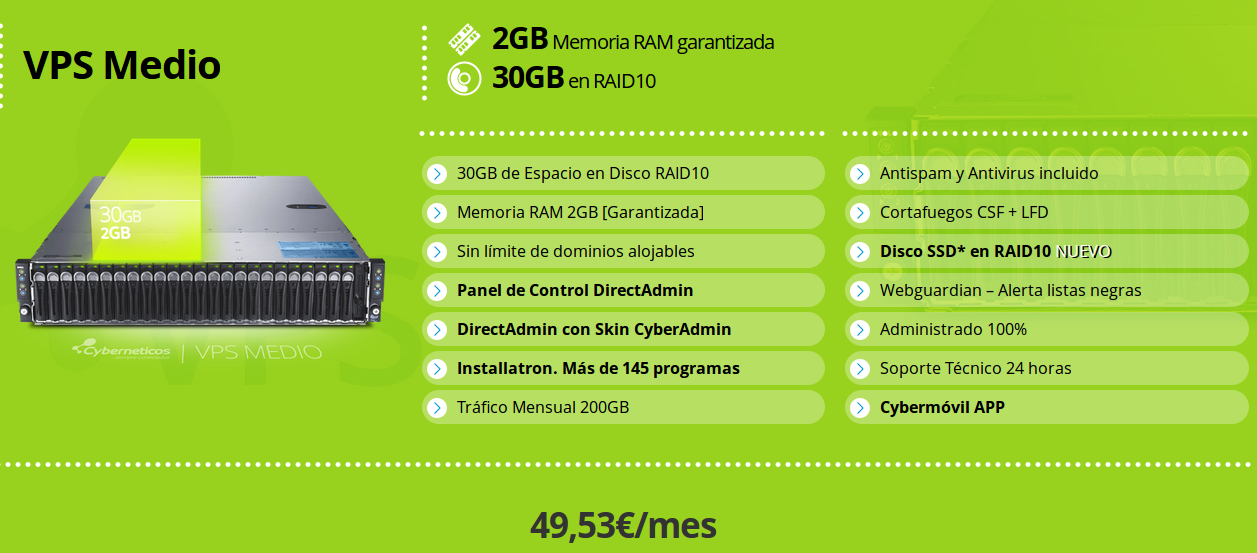
\includegraphics[scale=0.3]{ejercicio2-cyberneticos-2.png} 
		\label{figura2} 
		
		\caption{Cyberneticos,VPS medio} 
	\end{figure}
	
	\begin{figure}[H] 
		\centering
		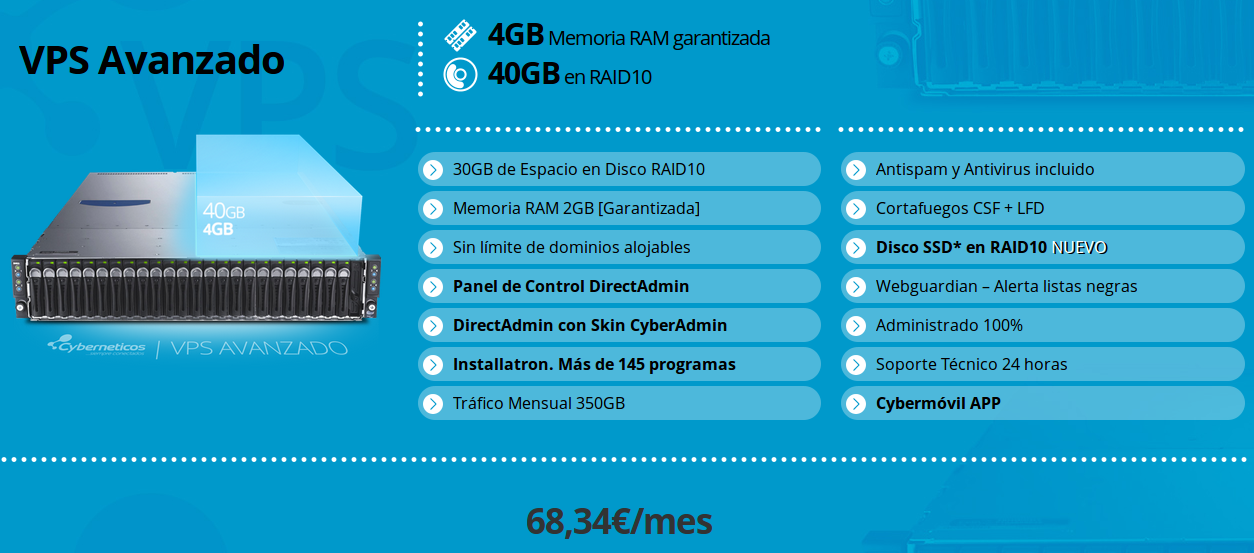
\includegraphics[scale=0.3]{ejercicio2-cyberneticos-3.png} 
		\label{figura3} 
		
		\caption{Cyberneticos,VPS avanzado} 
	\end{figure}
	
	\begin{figure}[H] 
		\centering
		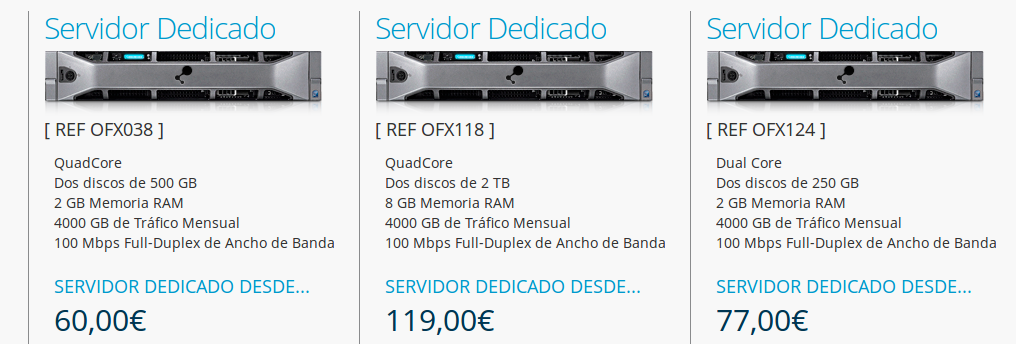
\includegraphics[scale=0.5]{ejercicio2-cyberneticos-4.png} 
		\label{figura4} 	
		\caption{Cyberneticos, servidores dedicados} 
	\end{figure}
	
		
	La empresa Dinahosting proporciona los siguiente servidores dedicados\cite{cincuentayseis}:
	
	
	\begin{figure}[H] 
		\centering
		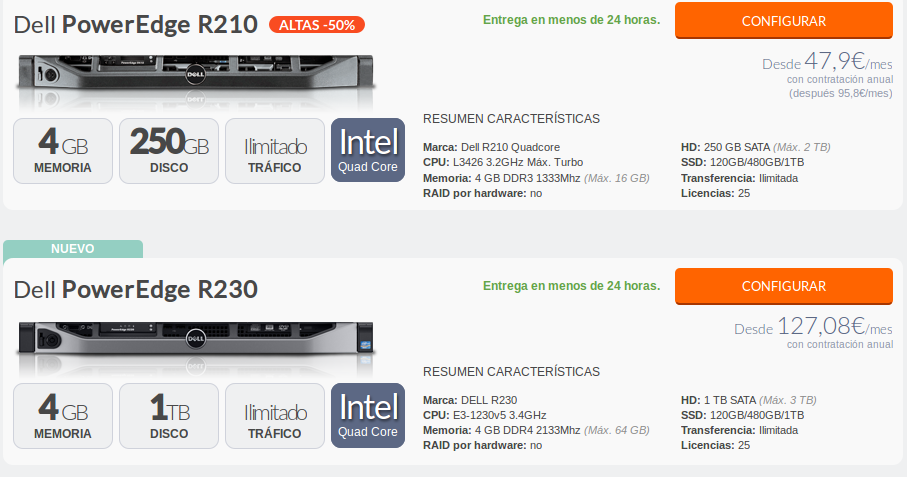
\includegraphics[scale=0.5]{ejercicio2-dinahosting-1.png} 
		\label{figura5} 	
		\caption{Dinahosting, servidores dedicados} 
	\end{figure}
	
	
	La empresa HostEuropa vende los siguientes VPS\cite{	cincuentaysiete} y servidores dedicados\cite{cincuentayocho}:


	\begin{figure}[H] 
		\centering
		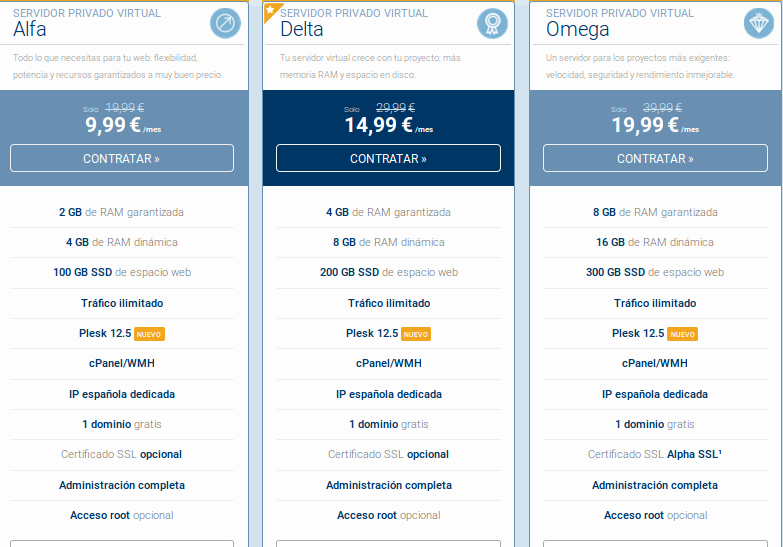
\includegraphics[scale=0.5]{ejercicio2-hosteuropa-1.png} 
		\label{figura6} 	
		\caption{HostEuropa, servidores VPS} 
	\end{figure}
	
	\begin{figure}[H] 
		\centering
		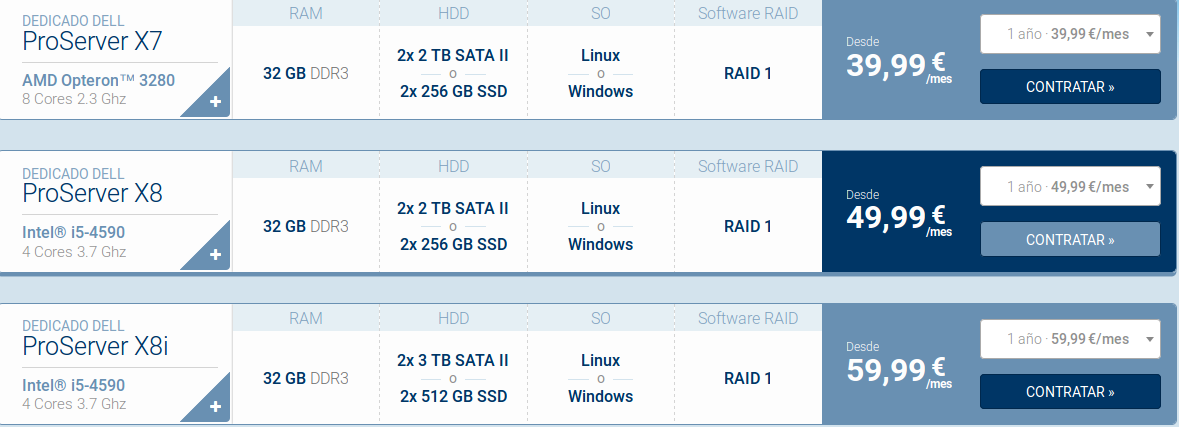
\includegraphics[scale=0.5]{ejercicio2-hosteuropa-2.png} 
		\label{figura7} 	
		\caption{HostEuropa, servidores dedicados} 
	\end{figure}
	
	%La siguiente tabla (Tabla \ref{tab:cyberneticos}) \footnote{http://www.cyberneticos.com/} muestra los productos de una empresa:
	
	%----------------Tabla 1--------------------------------
	%\begin{table}[H]
	%	\centering
	%	\scriptsize 
	%	\begin{tabular}{|c|c|c|c|c|c|}
	%		\hline
	%		{\bf Tipo} & {\bf Nombre} & {\bf Almacenamiento} & {\bf Memoria} & {\bf Procesador} & {\bf Precio} \\
	%		\hline
	%		VPS & VPS Básico & 20GB & 1GB & - & 35,31 euros/mes \\
	%		VPS & VPS Avanzado & 40GB & 4GB & - & 68,34 euros/mes \\
	%		Dedicado & - & 500GB & 4GB & QuadCore & 72 euros/mes \\
	%		Dedicado & - & 2x500GB & 8GB & QuadCore & 85 euros/mes \\
	%		\hline
	%	\end{tabular}  
	%	\caption{Comparativa empresa cyberneticos} \label{tab:cyberneticos}
	%\end{table}
	
	
	%La siguiente tabla (Tabla \ref{tab:dinahosting}) \footnote{https://dinahosting.com/} muestra los productos de otra empresa:
	
	%----------------Tabla 2--------------------------------
	%\begin{table}[H]
	%	\centering
	%	\begin{tabular}{|c|c|p{4cm}|c|c|c|}
	%		\hline
	%		{\bf Tipo} & {\bf Nombre} & {\bf \small Almacenamiento} & {\bf Memoria} & {\bf Procesador} & {\bf Precio} \\
	%		\hline
	%		VPS & V-Server Pro & 120GB & 1GB & - & 45 euros/mes  \\
	%		VPS & V-Server Pro Plus & 120GB & 1,5GB & - & 53 euros/mes \\
	%		VPS & V-ServerElite & 200GB & 2GB & - & 71 euros/mes \\
	%		Dedicado & Dell R200 & CPU:X3350, 2.66/2.83GHz & 2GB DDR2 & 1xQuadCore & 40 euros/mes \\
	%		Dedicado & Dell R210 & CPU:L3426 3.2GHz & 4GB DDR3 & 1xQuadCore & 47 euros/mes \\
	%		Dedicado & Dell R220 & CPU:E3-1230v3 3.3GHz & 4GB DDR2 & 1xQuadCore & 127 euros/mes \\
	%		\hline
	%	\end{tabular}  
	%	\caption{Comparativa empresa dinahosting} \label{tab:dinahosting}
	%\end{table}
	
	%Esta última tabla (Tabla \ref{tab:hosteurope}) \footnote{https://www.hosteurope.es/} muestra los productos de una tercera empresa:
	
	%----------------Tabla 3--------------------------------
	%\begin{table}[H]
	%	\centering
	%	\begin{tabular}{|c|c|c|c|c|c|}
	%		\hline
	%		{\bf Tipo} & {\bf Nombre} & {\bf Almacenamiento} & {\bf Memoria} & {\bf Procesador} & {\bf Precio} \\
	%		\hline
	%		VPS & ALFA & 200GB & 4GB & - & 9,74 euros/mes \\
	%		VPS & DELTA & 400GB & 8GB & - & 19,49 euros/mes \\
	%		VPS & OMEGA & 600GB & 16GB & - & 19,49 euros/mes \\
	%		Dedicado & ALFA & 2x1TB NL SAS 7.200 RPM & 8GB DDR3 & Intel Xeon E3-1230 & 64,99 euros/mes \\
	%		Dedicado & GAMMA & 2x2TB NL SAS 7.200 RPM & 16GB DDR3 & Intel Xeon E3-1240 & 77,99 euros/mes \\
	%		Dedicado & OMEGA & 2 x 600GB SAS 15.000 RPM & 32GB DDR3 & Intel Xeon E3-1270 & 77,99 euros/mes \\
	%		\hline
	%	\end{tabular}  
	%	\caption{Comparativa empresa hosteurope} \label{tab:hosteurope}
	%\end{table}
	
	Se puede ver que los servidores dedicados son vendidos con mejores características y que su precio es superior al de los VPS.
	
	
	%----------------------------------------------------------------------------------------
	%	Cuestión 3
	%----------------------------------------------------------------------------------------
	
	\section{a) Enumere y explique brevemente al menos tres de las innovaciones en Windows Server 2016 y 2012 R2 respecto a 2008R2. b) ¿Qué es Windows Server 2016 nano?}
	
	
	\subsection{a) Enumere y explique brevemente al menos tres de las innovaciones en Windows Server 2016 y 2012 R2 respecto a 2008R2.}
	
	En la siguiente comparativa de Microsoft\cite{segundo} podemos ver las mejoras de Windows Server 2016, Windows Server 2012 R2 y Windows Server 2008 R2. Algunas de ellas son:
	
	\begin{itemize}
		\item Innovaciones solo disponibles en Windows Server 2016:
		\begin{itemize}
			\item \textbf{Credential Guard\cite{tercero}(Protector de Credenciales}): Usa la seguridad basada en la virtualización para aislar información secreta que solo se puedan acceder a ellos de forma privilegiada.
			Un proceso de LSA (Local Security Authority) en el sistema operativo se comunica con un nuevo componente llamado proceso LSA aislado que almacena y protege los datos. Los datos almacenados mediante el proceso LSA aislado está protegidos mediante la seguridad basada en la virtualización y no es accesible para el resto del sistema operativo. LSA utiliza llamadas a procedimiento remoto para comunicarse con el proceso de LSA aislado.
			\item \textbf{Network Controller\cite{cuarto} (Controlador de Red):} Esta es una función de un servidor de alta disponibilidad y escalabilidad. Proporciona una API (interfaz de programación de aplicaciones) que permite a los controladores de red comunicarse con la red, y una segunda API que te permite comunicarte con el Controlador de Red.
		\end{itemize}
		\item Innovaciones disponibles con soporte completo o limitado en Windows Server 2012 R2 y soporte completo en Windows Server 2016:
		\begin{itemize}
			\item \textbf{Data deduplication\cite{quinto} (Deduplicación de Datos):} Consiste en encontrar y eliminar la duplicación dentro de los datos sin comprometer su integridad o fidelidad. Su objetivo es almacenar más datos en menos espacio mediante la segmentación de los archivos en pequeños trozos de tamaño variable, la identificación de fragmentos duplicados y el mantenimiento de una sola copia de cada trozo. Las copias redundantes del trozo se sustituyen por una referencia a una única copia. Los trozos son comprimidos y organizados en archivos de contenedor especiales en la carpeta System Volume Information (Información del Volumen del Sistema).
		\end{itemize}
	\end{itemize}
	
	\subsection{b) ¿Qué es Windows Server 2016 nano?}
	
	Encontramos información acerca de lo que es Windows Server 2016 nano\cite{sexto}, una incorporación reciente a su nueva gama de servidores.
	
	Un Servidor Nano es un servidor administrado de forma remota, optimizado para las nubes privadas y centros de datos. Es similar a Windows Server respecto al núcleo, pero más pequeño, sin capacidad local inicio de sesión, solo soporta aplicaciones de 64 bits, herramientas y agentes. Ocupa poco espacio en disco, se ejecuta más rápido y requiere menos actualizaciones y reinicios que Windows Server. Es ideal para varios casos, como por ejemplo:
	
	\begin{itemize}
		\item Como servidor DNS.
		\item Como servidor web con Servicios de Información de Internet.
		\item Como host para máquinas virtuales Hyper-V\cite{septimo}, permitiendo crear y administrar entornos informáticos virtualizados. 
	\end{itemize}
	

	%	Cuestión 4
	%-----------------------------------------------
	\section{¿Qué son los productos MAAS y Landscape ofrecidos por Canonical (la empresa que desarrolla Ubuntu)?}
	
	
	MAAS (Metal as a Service)\cite{octavo,noveno} es un servicio que ofrece un estilo de nube suministrado para servidores físicos. Este servicio ofrece la instalación más rápida en la industria gracias a su instalador con una base optimizada. Establece el RAID y la configuración de red que tu quieras a través de la web MAAS con interfaz de usuario o como cliente. Con MAAS, tu hardware puede ser parte de tu infraestructura de trabajo en cuestión de minutos. Da nueva vida a tu hardware viejo reciclándolo para usar en otras partes de tu red. Funciona con todos los servidores de certificados de cualquier proveedor importante,  lo que evita costosas actualizaciones y los proveedores de tecnología.
	\\
	
	Landscape\cite{decimo} es una herramienta de gestión con la cual podrás gestionar, monitorizar y desplegar tus servidores Ubuntu. Es la mejor forma de dar soporte y monitorizar redes de escritorio, servidores y nube grandes o en crecimiento respecto a efectividad y coste. Puedes controlar tu inventario así como gestionar repositorios de paquetes. Contiene Autopilot, un software para desplegar fácilmente una infraestructura de nube con OpenStack. 
	
	%----------------------------------------------------------------------------------------
	%	Cuestión 5
	%----------------------------------------------------------------------------------------
	
	\section{¿Qué relación tiene esta distribución con Red Hat y con el proyecto Fedora?}
	
	El proyecto Fedora\cite{once} fue patrocinado por Red Hat en septiembre de 2003, ya que invirtió en él para su desarrollo. Entre ambas se ayudan a promover el software libre. Fedora tiene empleados de Red Hat, así como una amplia comunidad de contribuidores y voluntarios. Para un seguimiento más exhaustivo, Fedora Project\cite{doce} nos dá información de la último década de trabajo conjunto.
	\\
	
	Fedora ahora es la base para distribuciones como Red Hat Enterprise Linux.
	Desde marzo de 2004, CentOS\cite{trece,catorce} fue apoyada por una comunidad que aportaba fuentes públicas por Red Hat. A partir de ese código libre se fue creando CentOS.
	\\
	
	CentOS utilizaba la parte de código libre de Red Hat Enterprise Linux (la que tiene licencia de GNU) para desarrollar CentOs.
	\\
	
	Finalmente en 2014 CentOS pasó a ser patrocinado por Red Hat, conteniendo cargos de junta de gobierno también de Red Hat.
	
	
	%----------------------------------------------------------------------------------------
	%	Cuestión 6
	%----------------------------------------------------------------------------------------
	
	\section{¿Qué diferencias hay entre RAID mediante SF y mediante HW?}
	
	Obtenemos información a través de una la empresa Adaptec\cite{quince} que es una fabricante de hardware.
	\begin{itemize}
		\item RAID software: La tarea del RAID se ejecuta en la CPU del sistema. Utiliza potencia de cálculo de CPU y el código del RAID se ejecuta en la CPU, compartiendo potencia de cálculo con el sistema operativo. Es vulnerable y suele tener problemas de integridad de datos.
		Se puede implementar de 2 formas:
		\begin{itemize}
			\item Como SW puro. El RAID se ejecuta en el host sin ningún tipo de hardware. Poco costoso, por estar integrado en el sistema operativo. No protege datos en el arranque. 
			\item Como solución híbrida con un poco de HW, para aumentar rendimiento y reducir sobrecarga CPU. Protección de datos en el arranque.
		\end{itemize}
		\item RAID hardware: Contiene su propia memoria y procesador para trabajar sobre el RAID.El RAID es independiente del SO, ya no depende tanto del sistema operativo como el RAID software. Son más fiables ya que aseguran la protección de datos que el RAID software no hacía. Por ejemplo protección en el arranque y no vulnerable.
		Tiene dos tipos de implementaciones:
		\begin{itemize}
			\item Como tarjeta controladora. 
			\item Hardware integrado: En un chip se encuentra integrado casi todo el hardware que contiene dicho RAID hardware.
		\end{itemize}
	\end{itemize}
	
	%----------------------------------------------------------------------------------------
	%	Cuestión 7
	%----------------------------------------------------------------------------------------
	\section{a) ¿Qué es LVM?  b) ¿Qué ventaja tiene para un servidor de gama baja? c) Si va a tener un servidor web, ¿le daría un tamaño grande o pequeño a /var?}
	
	\subsection{a)¿Qué es LVM?}
	
	LVM\cite{dieciseis,diecisiete,dieciocho}  (Logical Volumen Manager) es un administrador de volúmenes lógicos para Linux. Proporciona una mejor visión del almacenamiento en disco (uso de device-mapper), con más complejidad, detalles, redimensión de volúmenes y administrar grupos hechos por el usuario.En LVM se diferencian estos bloques:
	\begin{itemize}
		\item Volumen físico: Partición de disco duro que contiene grupos de volúmenes.
		\item Grupo de volúmenes: Varios volúmenes físicos usados para almacenamiento. Estos contienen a su vez volúmenes lógicos.
		\item Volumen lógico: Partición lógica que está en un grupo de volúmenes y contiene extensiones físicas.
		\item Extensión física: Menor tamaño de volumen físico que se asigna a uno lógico.
	\end{itemize}
	
	\subsection{b) ¿Qué ventaja tiene para un servidor de gama baja?}
	Para un servidor de baja gama, el cual no tiene el potencial de uno de alta, podría pasar que tuviese espacio insuficiente almacenar los datos que le podrían llegar debido a que se conectan bastantes clientes o las operaciones que realiza son bastantes costosas en cuanto a memoria y CPU.
	\\
	
	LVM ayuda a estos servidores ya que permite tomar decisiones sobre las particiones evitando que el almacenamiento de sus sistemas esté lleno por completo. Para ello usamos una reasignación de espacio\cite{diecinueve,veinte} , quitando memoria no usada de un sistema a otro que esté lleno. De este modo obtenemos mayor rendimiento del servidor al permitir una mayor gestión de información en caso de necesitarlo.
	
	\subsection{c) Si va a tener un servidor web, ¿le daría un tamaño grande o pequeño a /var?}
	El sistema de archivos /var contiene datos que cambian cuando el sistema se ejecuta normalmente \cite{veintiuna} . Es específico para cada sistema y no compartible.
	\\
	
	Para un servidor se necesitará de un tamaño grande\cite{veintidos}, sobre todo debido a /var/tmp, donde residen archivos temporales grandes y a /var/log que contiene archivos con información de login que pueden crecer mucho. También sostiene contenido de un número de aplicaciones, incluyendo el servidor web Apache. Este directorio además almacena paquetes de actualización descargados de forma temporal. Esta es una razón de más para poner espacio suficiente en /var.
	
	
	%----------------------------------------------------------------------------------------
	%	Cuestión 8
	%----------------------------------------------------------------------------------------
	\section{¿Debemos cifrar también el volumen que contiene el espacio para swap? ¿Y el volumen en el que montaremos /boot?}
	
	El espacio de swap si debe cifrarse\cite{veintitres}, ya que al cifrar particiones dicha clave se almacena en RAM.  Si hibernas tu equipo, los datos de RAM pasan a la partición de swap, por lo que si no la tienes cifrada podrían acceder a ella y robarte la clave.
	\\
	
	Leyendo detenidamente información de ArchLinux\cite{veinticuatro,veinticinco} encontramos información acerca de no cifrar /boot, no puede ser normalmente cifrada porque el gestor de arranque y BIOS no son capaces de desbloquear dm-crypt\cite{veintiseis}(Device-mapper es la infraestructura en el kernel de Linux cuyo objetivo es proporcionar cifrado transparente de los dispositivos de bloque utilizando una API de criptografía de kernel. Es el encargado de cifrar las particiones del sistema), con el fin de continuar con el proceso de arranque. 
	\\
	
	Una excepción sería GRUB, que consigue desbloquear un LUKS \cite{veintisiete}(Linux Unified Key Setup. Es una especificación para el cifrado de dispositivo de bloque. Establece un formato en disco para los datos, así como una política de gestión de los características de la contraseña o clave. Utiliza el subsistema de mapeador de dispositivos del núcleo a través del módulo dm-crypt). 
	\\
	
	La conclusión es no cifrar /boot, ya que si lo haces no podrías arrancar el sistema debido a que es la partición de arranque.
	
	
	%----------------------------------------------------------------------------------------
	%	Cuestión 9
	%----------------------------------------------------------------------------------------
	\section{¿a)Imagine que tiene un disco híbrido con tecnología SSD ¿Qué puntos de montaje ubicaría en este? b) Justifique qué tipo de sistema de archivos usaría para tener un servidor de streaming}
	
	\subsection{a) Imagine que tiene un disco híbrido con tecnología SSD ¿Qué puntos de montaje ubicaría en este?}
	
	En Linux vamos a tener diferentes puntos de montaje\cite{veintiocho,veintinueve}:
	
	\begin{itemize}
		\item \textbf{/ ó /root:} Directorio más alto de la jerarquía donde los principales sistemas de archivos son montados y desde el cual otros sistemas de archivos son montados. Debe tener contenidos adecuados para arrancar, restaurar y/o reparar el sistema. Esta partición es la más importante y necesaria. Contiene el directorio /usr, el cual crece dependiendo del software que tengas instalado.
		\item \textbf{/boot:} Contiene imágenes del núcleo y de RAM, así como el archivo de configuración del gestor de arranque. También almacena los datos son usados antes de que el núcleo empiece a ejecutar programas en espacio de usuario. 
		Esta partición no es necesaria para el funcionamiento normal del sistema, pero sí durante el arranque del kernel y sus actualizaciones.
		\item \textbf{/home:} Este directorio contiene archivos de configuración específica para el usuario, caches, datos de aplicaciones y archivos multimedia.
		\item \textbf{/var:} Almacena datos de variables de archivos y directorios, datos para administración e inicio de sesión. Sus datos serán leidos o escritos frecuentemente.
		\item \textbf{/data:} Se puede considerar esta partición para que varios archivos sean compartidos por todos los usuarios. El uso de la partición /home para este fin estaría bien también.
		\item \textbf{/tmp:} Es ya una partición separada por defecto, gracias a que es montada como tmpfs por systemd por lo que no hay necesidad de crear una partición para ello.
		\item \textbf{swap:} Proporciona memoria que se puede utilizar como RAM virtual. Tiene archivos de intercambio que pueden cambiar su tamaño según sea necesario.
		\item \textbf{/bin\cite{treinta}:} Contiene binarios esenciales y ejecutables.
		\item \textbf{/dev\cite{treintayuno}:} Archivos de dispositivo.
		\item \textbf{/etc\cite{treintaydos}:} Configuración específica del host.
		\item \textbf{/usr\cite{treintaytres}:} Contiene grandes cantidades de información compartida en el sistema. Contiene cabeceras, binarios, su documentación, librerías,etc. 
	\end{itemize}
	
	Con la tecnología SSD tenemos diferentes mejoras, como describen por ejemplo  Intel\cite{treintaycuatro} y IBM\cite{treintaycinco} describe las suyas:
	
	\begin{itemize}
		\item Los disco duros de estado sólido no tienen piezas móviles, al contrario que los discos duros tradicionales (HDD) que utilizan un brazo mecánico para mover y leer la información en discos giratorios.
		\item Utilizan memoria no volátil, aquella que aunque se apague la información guardada no se pierde.
		\item Los de Intel tienen protección de punto a punto, para proteger los datos.
		\item Mejoras significantes en rendimiento.
		\item Pueden estar casi llenos y seguir al mismo rendimiento, sin degradarse.
		\item Tiempos de acceso más rápidos.
		\item Uso reducido de energía.
	\end{itemize}
	
	Según Debian\cite{treintayseis}, la memoria SSD acelera la parte estática del sistema y el trabajo de datos importantes del usuario. Por lo tanto, considera que la mejor opción es usarla en /root.
	
	Así mismo, Ubuntu\cite{treintaysiete} aconseja que lo mejor sería dejar todos los archivos de solo lectura en el disco SSD y usar el disco duro para todo lo demás. Se puede ver como hace referencia a un contenido donde explica que partes del sistema de archivos pueden ser de solo lectura, llegando a explicar como habilitar /root para ello.
	\\
	
	Como conclusión, una vez explicada la funcionalidad de /root y los consejos semejantes de Debian y Ubuntu a la hora de hacer un punto de montaje en un SSD, concluyo que la mejor opción\cite{treintayocho} es tener la SSD dentro de los directorios /bin que contiene información básica de programas, por lo que se harán lecturas en él, /usr el cual contiene mas binarios del sistema, siendo su lectura necesaria para que funcione el sistema, /dev; incluso /home y /data. 
	
	\subsection{b) Justifique qué tipo de sistema de archivos usaría para tener un servidor de streaming}
	
	Según Red Hat, en su informe blanco o documento con autoridad\cite{treintaynueve} (whitepaper) acerca de 'como elegir tu sistema de archivos de empresa Red Hat', se recomienda elegir el sistema de archivos XFS, ya que optimiza la carga de vídeo en streaming.
	\\
	
	XFS es un sistema de archivos robusto y maduro de journaling que soporta archivos muy grandes y sistema de archivos en una sola máquina. Más información sobre este curioso sistema de archivos puede ser encontrada en Red Hat\cite{cuarenta}
	
	%----------------------------------------------------------------------------------------
	%	Cuestión 10
	%----------------------------------------------------------------------------------------
	\section{Muestre como ha quedado el disco particionado una vez el sistema está instalado.(lsblk)}
	
	Podemos ejecutar el comando lsblk -l \cite{cuarentayuno} para mostrar información sobre los dispositivos de bloques:
	
	\begin{figure}[H] %con el [H] le obligamos a situar aquí la figura
		\centering
		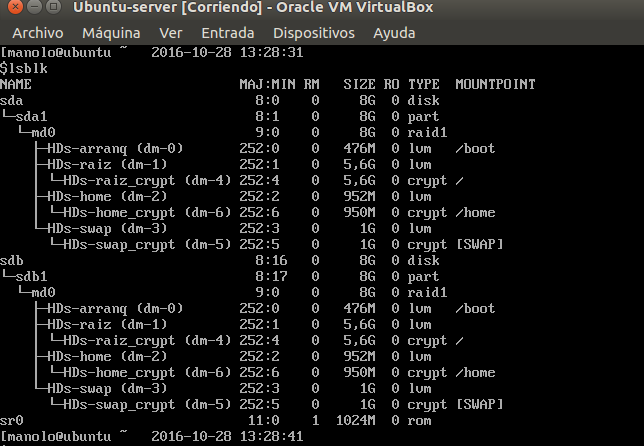
\includegraphics[scale=0.5]{ejercicio10.png}  %el parámetro scale permite agrandar o achicar la imagen. En el nombre de archivo puede especificar directorios
		\label{figura8} 
		
		\caption{Particionado de disco} 
	\end{figure}
	
	%----------------------------------------------------------------------------------------
	%	Cuestión 11
	%----------------------------------------------------------------------------------------
	\section{a) ¿Cómo ha hecho el disco 2 “arrancable”? b) ¿Qué hace el comando grub-install?}
	
	He probado a eliminar el disco 1 y efectivamente el sistema no puede arrancar debido a que el arranque se encuentra en el disco 1.
	
	\begin{figure}[H]
		\centering
		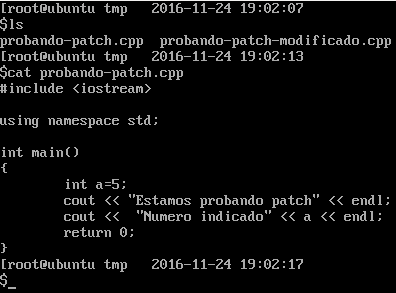
\includegraphics[scale=0.4]{ejercicio11-1.png} 
		\label{figura9} 		
		\caption{Eliminación de disco 1 de Ubuntu Server} 
	\end{figure}
	
	Podemos ver como el sistema no termina de arrancar.
	
	\begin{figure}[H]
		\centering
		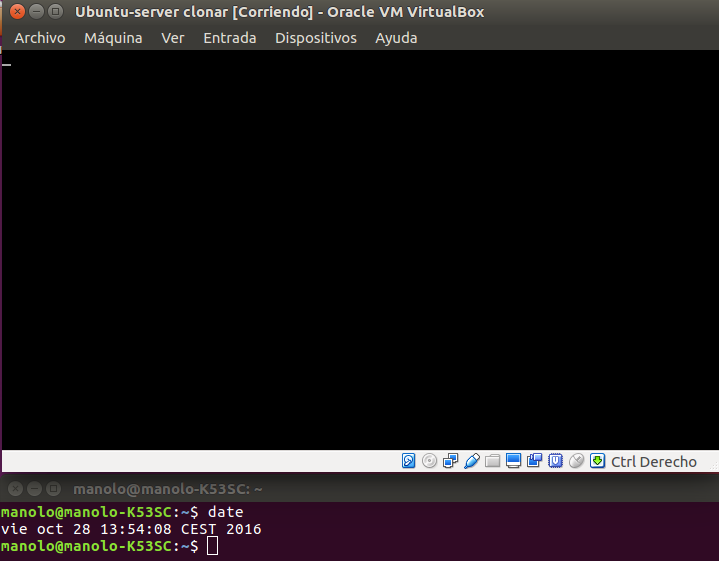
\includegraphics[scale=0.3]{ejercicio11-2.png} 
		\label{figura10} 		
		\caption{Comprobación de arranque de Ubuntu Server sin disco 1} 
	\end{figure}
	
	\subsection{a) ¿Cómo ha hecho el disco 2 “arrancable”?} 
	
	Para que sea arrancable el disco 2 debe instalarse GRUB\cite{cuarentaydos,cuarentaytres,cuarentaycuatro}. Se hace con el comando sudo grub-install /dev/sdb \cite {cuarentaycinco}. Gracias a la instalación del gestor de arranque podemos seleccionar la partición desde la que arrancar el sistema, permitiendo arrancar desde el disco 2.
	
	\begin{figure}[H]
		\centering
		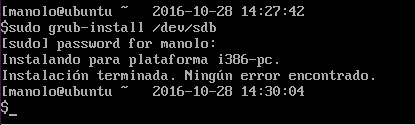
\includegraphics[scale=0.6]{ejercicio11-3.png} 
		\label{figura11} 		
		\caption{Instalación de GRUB en el disco 2 con grub-install} 
	\end{figure}
	
	Comprobamos que ahora deje arrancar con el disco 2. Para ello primero borramos el disco 1 y después arrancamos el sistema.
	
	\begin{figure}[H]
		\centering
		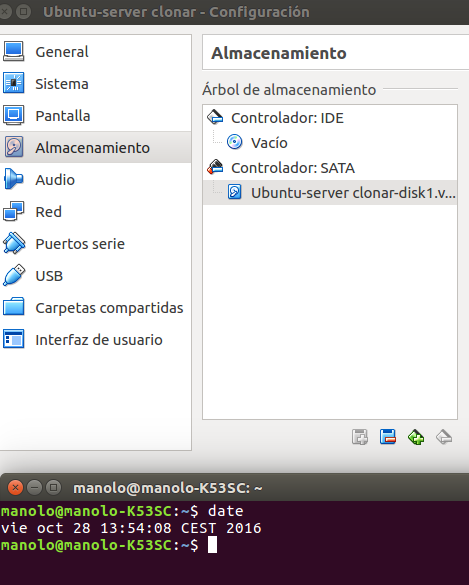
\includegraphics[scale=0.4]{ejercicio11-4.png} 
		\label{figura12} 		
		\caption{Borrado de disco 1 tras instalarle GRUB} 
	\end{figure}
	
	\begin{figure}[H]
		\centering
		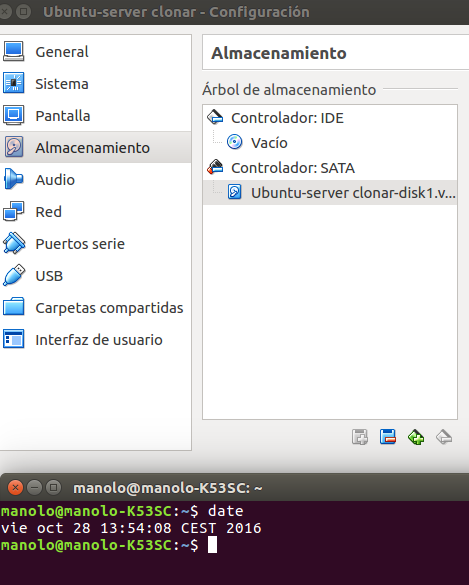
\includegraphics[scale=0.4]{ejercicio11-4.png} 
		\label{figura13} 		
		\caption{Borrado de disco 1 tras instalarle GRUB} 
	\end{figure}
	
	Ahora vemos como nos sale el GRUB al iniciar.
	
	\begin{figure}[H]
		\centering
		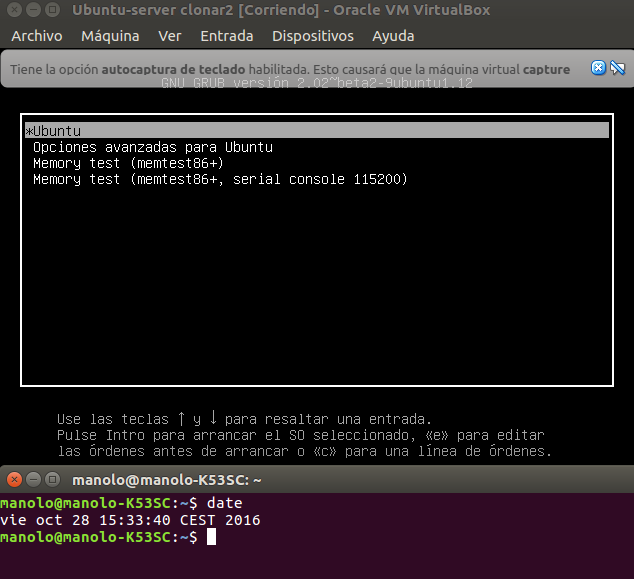
\includegraphics[scale=0.4]{ejercicio11-5.png} 
		\label{figura14} 		
		\caption{Visualización de GRUB tras borrado de disco 1} 
	\end{figure}
	
	Parece que hay problemas o algún bug al arrancar el disco 2, como consecuencia de detectar que uno de los disco ha sido extraído. Podemos verlo con cat /proc/mdstat \cite{cuarentaysiete}.
	
	\begin{figure}[H]
		\centering
		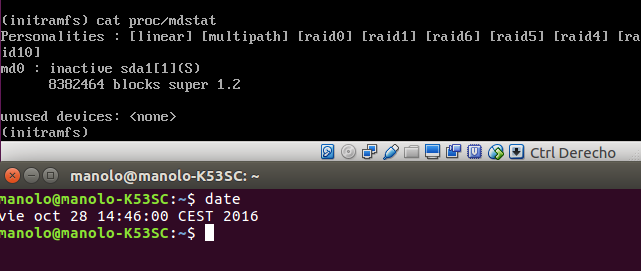
\includegraphics[scale=0.4]{ejercicio11-6.png} 
		\label{figura15} 		
		\caption{Error de disco 2 con GRUB} 
	\end{figure}
	
	Podemos solucionarlo con mdadm -R /dev/md0\cite{cuarentayocho}.
	
	\begin{figure}[H]
		\centering
		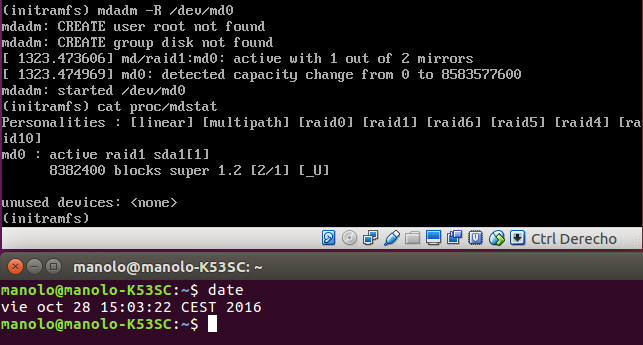
\includegraphics[scale=0.3]{ejercicio11-7.png} 
		\label{figura16} 		
		\caption{Solución error de disco 2 con GRUB} 
	\end{figure}
	
	De este modo ya funciona Ubuntu Server.
	
	\begin{figure}[H]
		\centering
		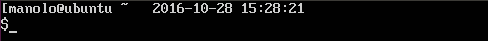
\includegraphics[scale=0.5]{ejercicio11-8.png} 
		\label{figura17} 		
		\caption{Ubuntu Server ejecutándose con disco 2} 
	\end{figure}
	
	\subsection{b) ¿Qué hace el comando grub-install?}
	
	Grub-install\cite{cuarentayseis}  hace lo siguiente según el manuel de Linux: instala grub en su unidad, install-device puede ser un nombre de dispositivo GRUB o un nombre de archivo de dispositivo del sistema. Copia la imagen de GRUB en el directorio DIR/boot especificado por el directorio -root-, y utiliza el Shell de grub para instalar GRUB en el sector de arranque.
	
	
	
	
	
	%----------------------------------------------------------------------------------------
	%	Cuestión 12
	%----------------------------------------------------------------------------------------
	
	\section{¿Qué diferencia hay entre Standard y Datacenter?}
	
	Datacenter\cite{cuarentaynueve}  sirve para entornos virtualizados ya que permite ejecutar muchas máquinas virtuales en dos procesadores, mientras que Standard sirve para entornos poco virtualizados por el hecho de permitir solo dos máquinas virtuales en dos procesadores.
	%----------------------------------------------------------------------------------------
	%	Cuestión 13
	%----------------------------------------------------------------------------------------
	\section{Continúe usted con el proceso de definición de RAID1 para los dos discos de 50MiB que ha creado. Muestre el proceso con capturas de pantalla.}
	
	\begin{itemize}
	\item \textbf{Primer paso:} Entrar el Administrador del servidor >    Administrador de discos.
	\end{itemize}
	
	\begin{figure}[H]
		\centering
		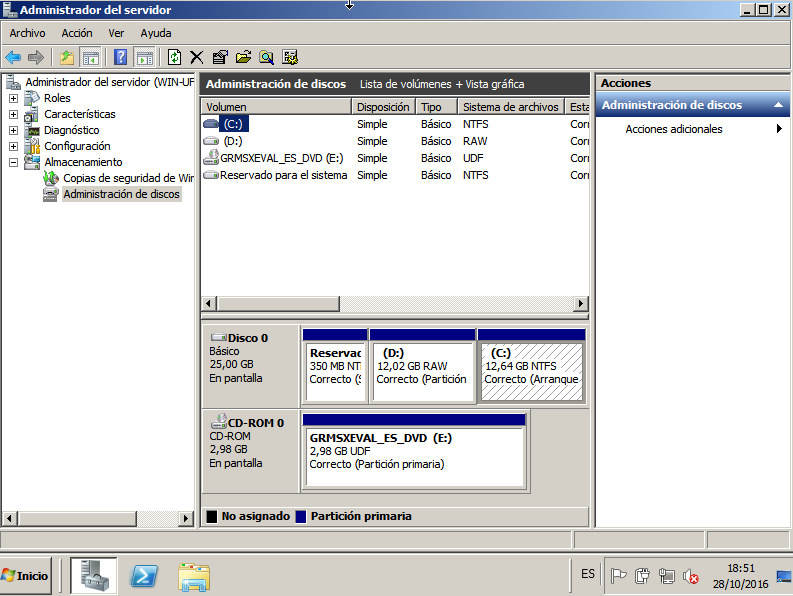
\includegraphics[scale=0.5]{ejercicio13-1.png}  
		\label{figura18}
		\caption{Entrar al administrador de discos} 
	\end{figure}
	
	
	\begin{itemize}
		\item \textbf{Segundo paso:}Inicializar los discos con MBR (Registro de arranque maestro).
	\end{itemize}
	
	\begin{figure}[H]
		\centering
		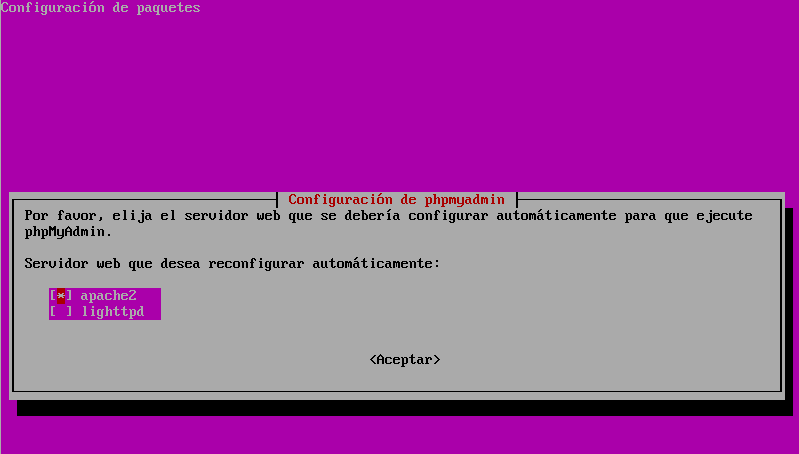
\includegraphics[scale=0.5]{ejercicio13-2.png}  
		\label{figura19}
		\caption{Inicializar los discos} 
	\end{figure}
	
	\begin{itemize}
		\item \textbf{Tercer paso:} Establecer un "Nuevo volumen reflejado" haciendo click derecho sobre el disco 1.
	\end{itemize}
	
	\begin{figure}[H]
		\centering
		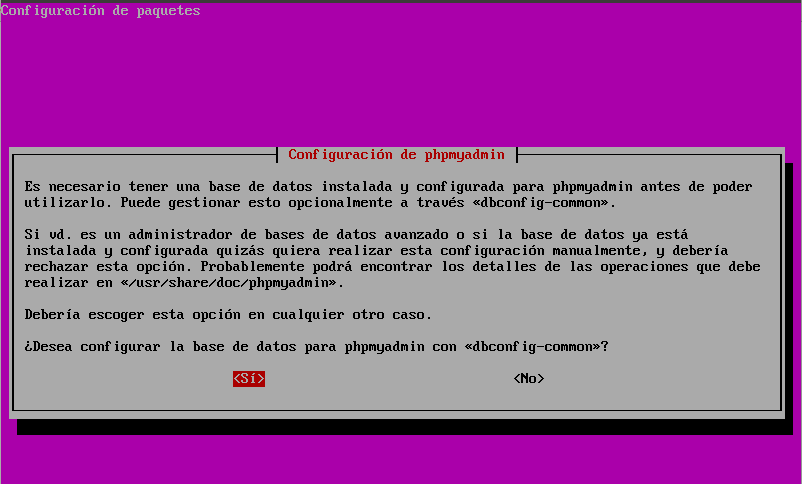
\includegraphics[scale=0.5]{ejercicio13-3.png}  
		\label{figura20}
		\caption{Nuevo volumen reflejado en disco 1} 
	\end{figure}
	
	\begin{itemize}
		\item \textbf{Cuarto paso:}Agregar disco para que pueda reflejar.
	\end{itemize}
	
	\begin{figure}[H]
		\centering
		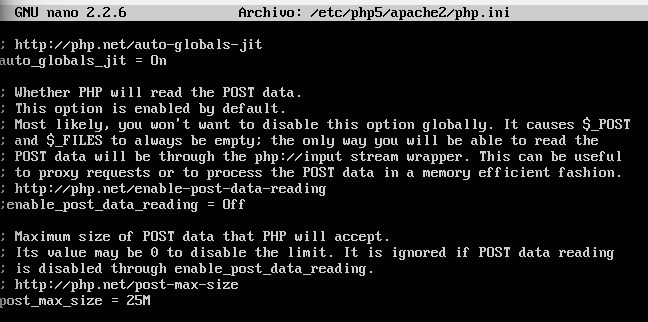
\includegraphics[scale=0.5]{ejercicio13-4.png}  
		\label{figura21}
		\caption{Agregar disco reflejado} 
	\end{figure}
	
	\begin{itemize}
		\item \textbf{Quinto paso:}Asignar letra de unidad o ruta de acceso al nuevo volumen fijado.
	\end{itemize}
	
	\begin{figure}[H]
		\centering
		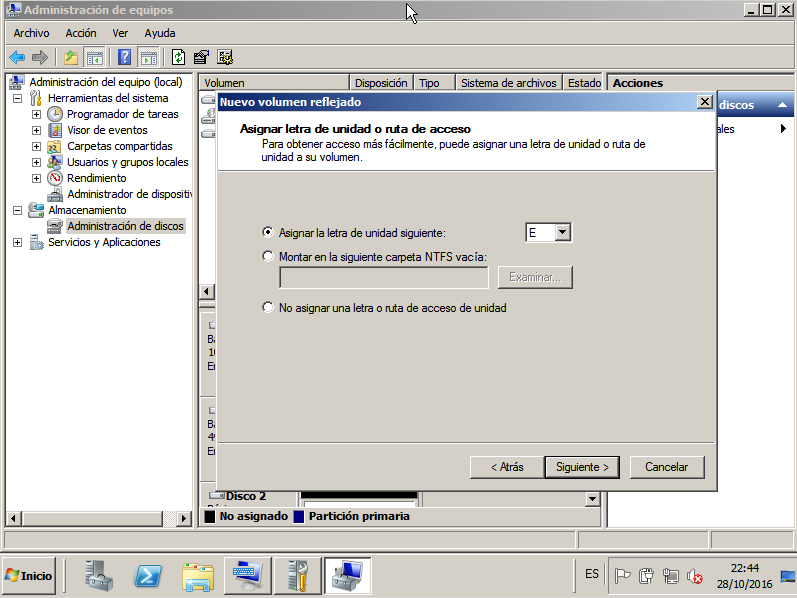
\includegraphics[scale=0.5]{ejercicio13-5.png}  
		\label{figura22}
		\caption{Asignar letra de unidad o ruta de acceso al nuevo volumen fijado} 
	\end{figure}
	
	\begin{itemize}
		\item \textbf{Sexto paso:} Formatear volumen, en NTF, con tamaño predeterminado y elegiendo el nombre que quieras.
	\end{itemize}
	
	\begin{figure}[H]
		\centering
		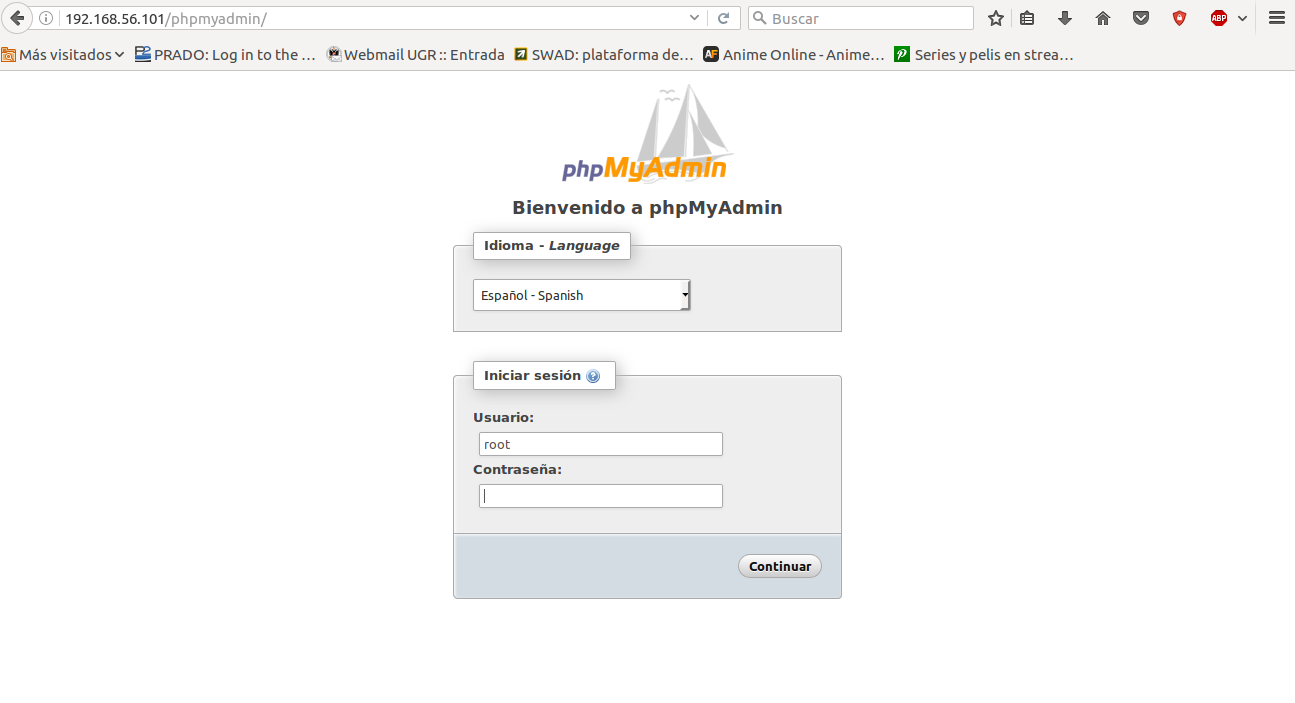
\includegraphics[scale=0.5]{ejercicio13-6.png}  
		\label{figura23}
		\caption{Formatear volumen reflejado} 
	\end{figure}
	
	\begin{itemize}
		\item \textbf{Séptimo paso:} Aceptar convertir los discos a dinámicos.
	\end{itemize}
	
	\begin{figure}[H]
		\centering
		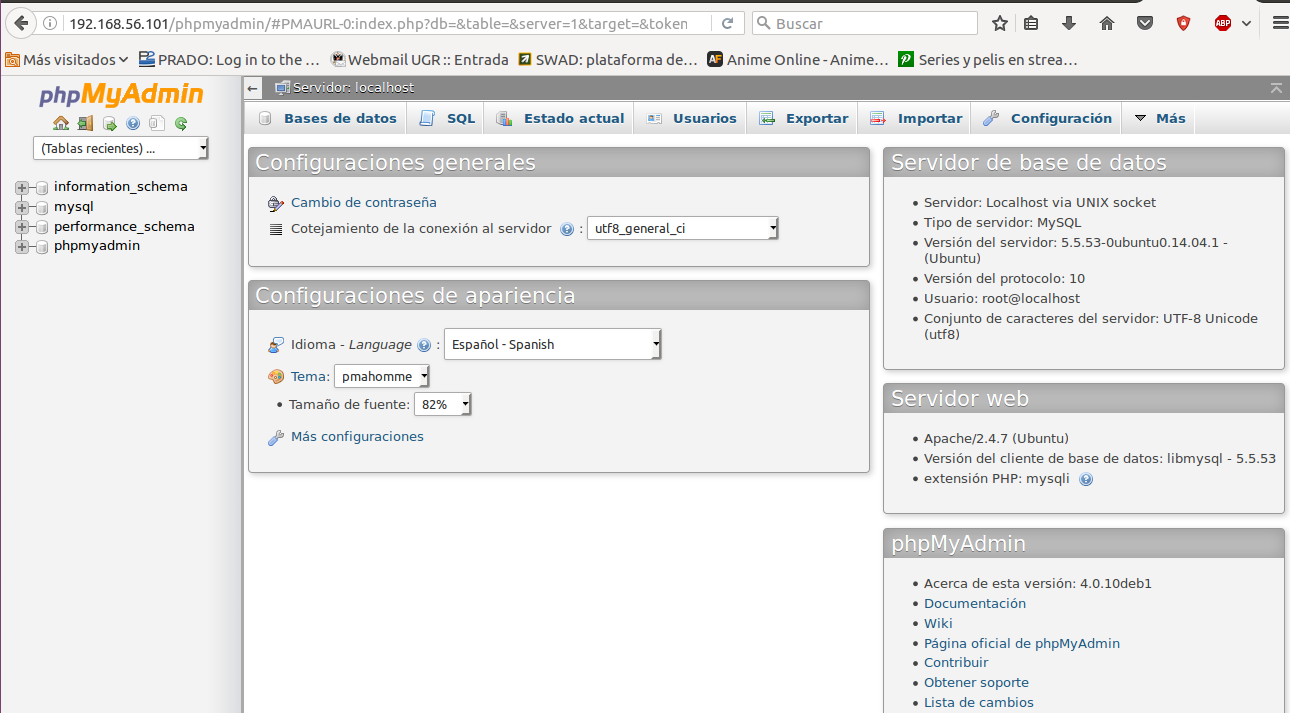
\includegraphics[scale=0.5]{ejercicio13-7.png}  
		\label{figura24}
		\caption{Aceptar convertir los discos a dinámicos} 
	\end{figure}
	
	\begin{itemize}
		\item \textbf{Octavo paso:} Mostrar que el RAID1 se ha hecho correctamente.
	\end{itemize}
	
	\begin{figure}[H]
		\centering
		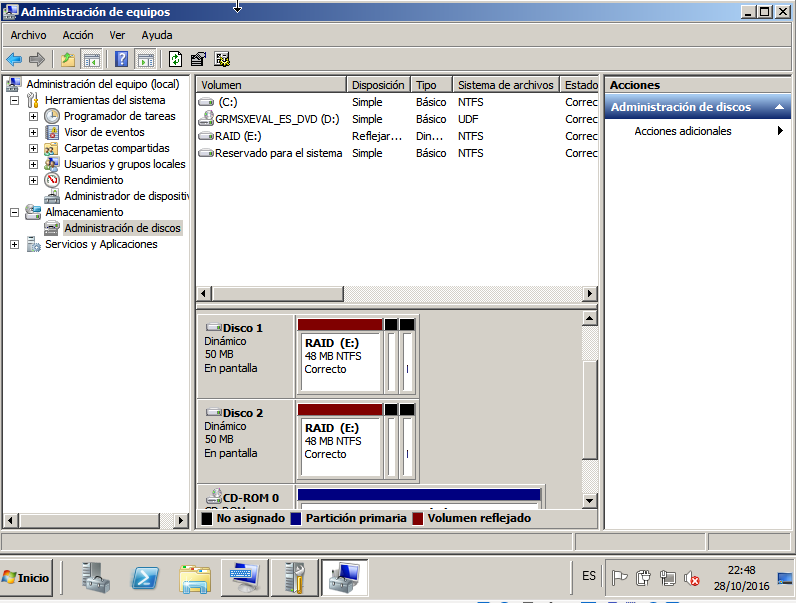
\includegraphics[scale=0.5]{ejercicio13-8.png}  
		\label{figura25}
		\caption{Visión de los discos tras el RAID1} 
	\end{figure}
	
	
	
	%----------------------------------------------------------------------------------------
	%	Cuestión 14
	%----------------------------------------------------------------------------------------
	
	\section{Explique brevemente qué diferencias hay entre los tres tipos de conexión que permite el VMSW para las Mvs: NAT, Host-only y Bridge.}
	
	Hemos encontrado información en un fabricante de VM, 
	WMware\footnote{https://www.vmware.com/}:
	
	\begin{itemize}
		\item Bridge\cite{cincuenta}: La máquina virtual se conecta a red por adaptador Ethernet de tu ordenador anfitrión. La máquina virtual será como un equipo más, independiente de la red.
		\item Nat\cite{cincuentaydos} (Network Address Translation): Da acceso a red usando la IP de tu equipo físico. Para comunicarse con la red, lo hace a través de un firewall.
		\item Host-Only\cite{cincuentaytres}: Red de la máquina virtual contenida en tu equipo por completo. Lógicamente la virtualización está en tu equipo.
	\end{itemize}
	
	%----------------------------------------------------------------------------------------
	%	Cuestión opcional 1
	%----------------------------------------------------------------------------------------
	\section{Opcional 1: Muestre (con capturas de pantalla) cómo ha comprobado que el RAID1 funciona.}
	
	Creamos 2 archivos dentro de /var y /home:
	
	\begin{figure}[H]
		\centering
		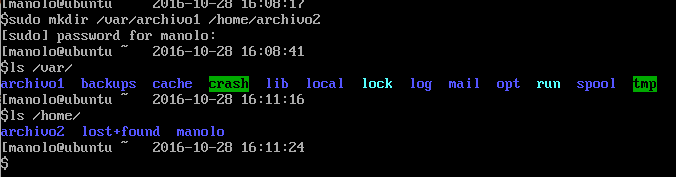
\includegraphics[scale=0.5]{opcional1-1.png}  
		\label{figura26}
		
		\caption{Creación de archivos en Ubuntu Server para comprobación RAID1} 
	\end{figure}
	
	
	Ahora vamos a forzar a un error en el disco 1(sda):
	
	\begin{figure}[H]
		\centering
		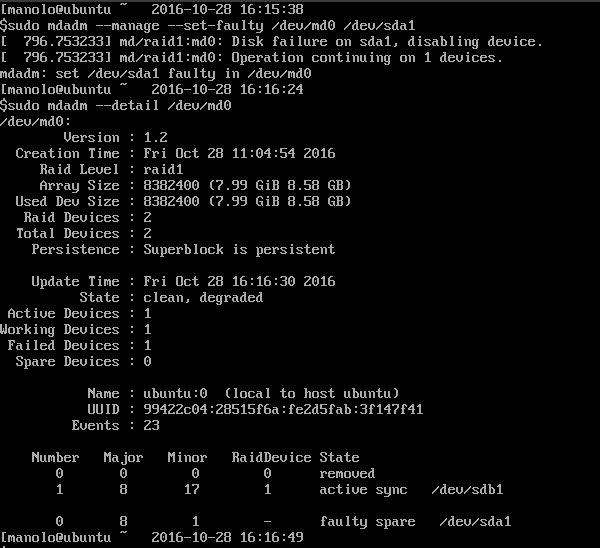
\includegraphics[scale=0.5]{opcional1-2.png}  
		\label{figura27}
		
		\caption{Forzar error de disco 1 para comprobación RAID1} 
	\end{figure}
	
	Podemos ver como pone que 'Operation continuing on 1 devices' lo que quiere decir que a pesar de que el disco 1 no sirva, el 2 sigue sirviendo y los datos se siguen conservando. Hay un campo que pone "Persistence : Superblock is persistent" lo que quiere decir la información se sigue manteniendo.
	\\
	
	Ahora vamos a desconectar el disco 1 y comprobar que nuestros archivos siguen estando disponibles:
	
	\begin{figure}[H]
		\centering
		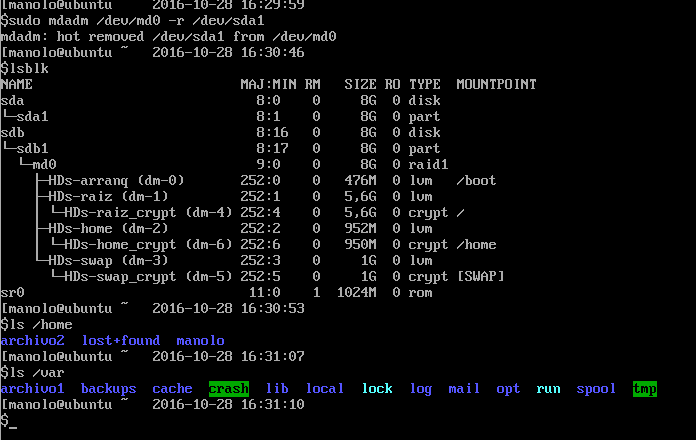
\includegraphics[scale=0.5]{opcional1-3.png}  
		\label{figura28}
		
		\caption{Desconexión de disco 1 y comprobación disponibilidad de los archivos creados} 
	\end{figure}
	
	Podemos ver que tras desconectar el disco 1, los archivos siguen estando como se muestra con la orden ls.
	%----------------------------------------------------------------------------------------
	%	Cuestión opcional 2
	%----------------------------------------------------------------------------------------
	\section{Opcional 2: ¿Qué relación hay entre los atajos de teclado de emacs y los de la consola bash? ¿y entre los de vi y las páginas del manual?}
	
	\subsection{¿Qué relación hay entre los atajos de teclado de emacs y los de la consola bash?}
	
	Podemos saber que ambos atajos son parecidos cuando por ejemplo movemos el cursor y además en la consola es parecido a bash, ya que ambos son parte del Proyecto GNU y además emacs está preparado para integrarse en bash\cite{cincuentaynueve,sesenta}:
	
	\begin{itemize}
		\item CTRL-B: Mover el cursor al carácter anterior.
		\item CTRL-F: Se mueve adelante de un carácter.
		\item CTRL-P: Vuelve a un comando anterior a bash y se mueve a la linea superior en emacs.
	\end{itemize}
	
	\subsection{¿y entre los de vi y las páginas del manual?}
	
	Podemos decir que ambos forman parte del proyecto GNU también y algunos atajos de vi\cite{sesentayuno,sesentaydos} son parecidos a los del manual. Por ejemplo:
	
	\begin{itemize}
		\item Al pulsar / y escribes algo que quieras buscar y pulsas enter, muestra la primera palabra escrita si hay. También usa n para pasar al siguiente.
		\item Usar 'd' y 'u' para avanzar media página hacía arriba o abajo.
		\item Pulsar q para salir.
		\item Pulsar h para la ayuda.
	\end{itemize}
	
	%------------------------------------------------
	

	

%------------------------------------------------

\bibliography{citas} %archivo citas.bib que contiene las entradas 
\bibliographystyle{plain} % hay varias formas de citar

\end{document}
